ATLAS (\textbf{A} \textbf{T}oroidal \textbf{L}HC \textbf{A}pparatu\textbf{S}) is a 
multi-purpose particle detector located at one of the 
LHC interaction points 100 meters underground. 
It is the largest particle detector ever built with a weight of about 7000 tonnes, a lenght of 44 m, 
and a diameter of 25 m as shown in Figure~\ref{fig:exp.atlas.atlas}.
It is designed to probe Higgs physics, QCD, flavour physics, as well as a multitude of beyond Standard Model (BSM) physics scenarios including supersymmetry.

ATLAS covers a solid angle of almost $4\omega$ to capture as much information from the collisions 
as possible. 
It is compsed of multiple layers of detectors to ensure that all particles produced in the 
collision are identified and measured with high accuracy.
These subsystems are shown in Figure~~\ref{fig:exp.atlas.atlas}.
The first detector resides in the part closest to the
LHC pipe and is composed of silicon tracking sensors designed to reconstruct the paths
of charged particles. 
Next, comes the electromagnetic and hadronic calorimeter cells that 
measure the energy of particles. Last comes the muon spectrometer in the outermost part of the 
detector to detect muons since they penetrate the calorimeters. 
An axial magnetic field of 2 T is applied across the inner detector while a toroidal magnetic field 
of approximately 0.5 T is applied across the muon detectors.
The remainder of this chapter will describe in more details these detectors.

\subsection{Co-ordinate System}

The common coordinate system of ATLAS is right-handed Cartesian, 
with its origin at the nominal interaction point. 
The axes are oriented such that the $x$-axis is pointing towards the centre of the LHC ring, the $y$-axis is directed
vertically upward, and the $z$-axis defines one of the beam directions.
The $(x, y)$ plane defines the transverse plane, usually represented by polar coordinates $(r,\phi)$
with $\phi=0$ on the $x$-axis.
The polar angle $\theta$ is replaced by the pseudorapidity
\begin{equation}
\eta = - \ln\left(\tan\left(\frac{\theta}{2}\right)\right).
\end{equation}
It is named after the rapidity since it yields the same quantity for massless particles
\begin{equation}
y = \frac{1}{2}\ln\left(\frac{E+p_Z}{E-p_Z}\right),
\end{equation}
which is invariant under boosts in the $z$-direction.
It is common to describe the separation between two physical objects in the detector by 
\begin{equation}
\Delta R = \sqrt{\Delta \eta^2 + \Delta \phi^2}
\end{equation}



\subsection{Inner detector}




\subsection{Calorimeters}

\subsection*{LAr Calorimeters}
\subsection*{Tile Calorimeters}


\subsection{Muon System}




\begin{figure}[t!]
\centering
\begin{subfigure}[t]{0.48\textwidth}
\includegraphics[width=0.95\textwidth]{sumLumiByDay}
\subcaption{Total Integrated Luminosity in 2016 }
\label{fig:exp.sumLumiByDay}
\end{subfigure}
\begin{subfigure}[t]{0.48\textwidth}
\includegraphics[width=0.95\textwidth]{recEffByWeek}
\subcaption{Data Taking Efficiency per Week in 2016}
\label{fig:exp.recEffByWeek}
\end{subfigure}
\vspace{-0.25cm}
\caption{(a) Cumulative luminosity versus time delivered to (green) and recorded by ATLAS (yellow) during stable beams for pp collisions at 13 TeV centre-of-mass energy in 2016. 
The recorded luminosity reflects the DAQ inefficiency, as well as the inefficiency of the so-called ``warm start'': when the stable beam flag is raised, the tracking detectors undergo 
a ramp of the high-voltage and, for the pixel system, turning on the preamplifiers.
(b) ATLAS data taking efficiency in 2016. The denominator is the luminosity delivered between the declaration of stable beams and the LHC request to turn the sensitive detectors off to allow a beam dump or beam studies. The numerator is the luminosity recorded by ATLAS. Each bin represents one day. The empty bins are due to days in which no stable beams were delivered by the LHC. The inefficiency accounts for the time needed to turn on the high-voltage of the Pixel, SCT, and some of the muon detectors at the start of an LHC fill and any inefficiencies due to deadtime or due to individual problems with a given sub detector that prevents the ATLAS data taking to proceed. }
\label{fig:exp.atlas.datarec}
\end{figure} 




\begin{figure}[t!]
\centering
\begin{subfigure}[t]{0.48\textwidth}
\includegraphics[width=0.95\textwidth]{peakLumiByFill}
\subcaption{Peak Luminosity per Fill in 2016}
\label{fig:exp.peakLumiByFill}
\end{subfigure}
\begin{subfigure}[t]{0.48\textwidth}
\includegraphics[width=0.95\textwidth]{peakMuByFill}
\subcaption{Peak Interactions per Crossing in 2016 }
\label{fig:exp.peakMuByFill}
\end{subfigure}
\vspace{-0.25cm}
\caption{(a) The peak instantaneous luminosity delivered to ATLAS during stable beams for pp collisions at 13 TeV centre-of-mass energy is shown for each LHC fill as a function of time in 2016. The luminosity is determined using counting rates measured by the luminosity detectors, and is based on a preliminary analysis of van-der-Meer beam-separation scans during 2016.
(b) The maximum number of inelastic collisions per beam crossing ($\mu$) during stable beams for pp collisions at 13 TeV centre-of-mass energy is shown for each fill in 2016. The preliminary luminosity measurement is used to determine the number of interactions per beam crossing as $mu = L_\text{bunch}  \sigma_\text{inel} / f_r$ where $L_\text{bunch}$ is the per-bunch instantaneous luminosity, $ \sigma_\text{inel} $ is the inelastic cross-section at 13 TeV, which is taken to be 80 mb, and $ f_r$ is the LHC revolution frequency of 11.245 kHz. The number of interactions shown is averaged over all colliding bunch pairs, and only the peak value per fill during stable beams is shown.
 }
\label{fig:}
\end{figure} 




\begin{figure}[t!]
\centering
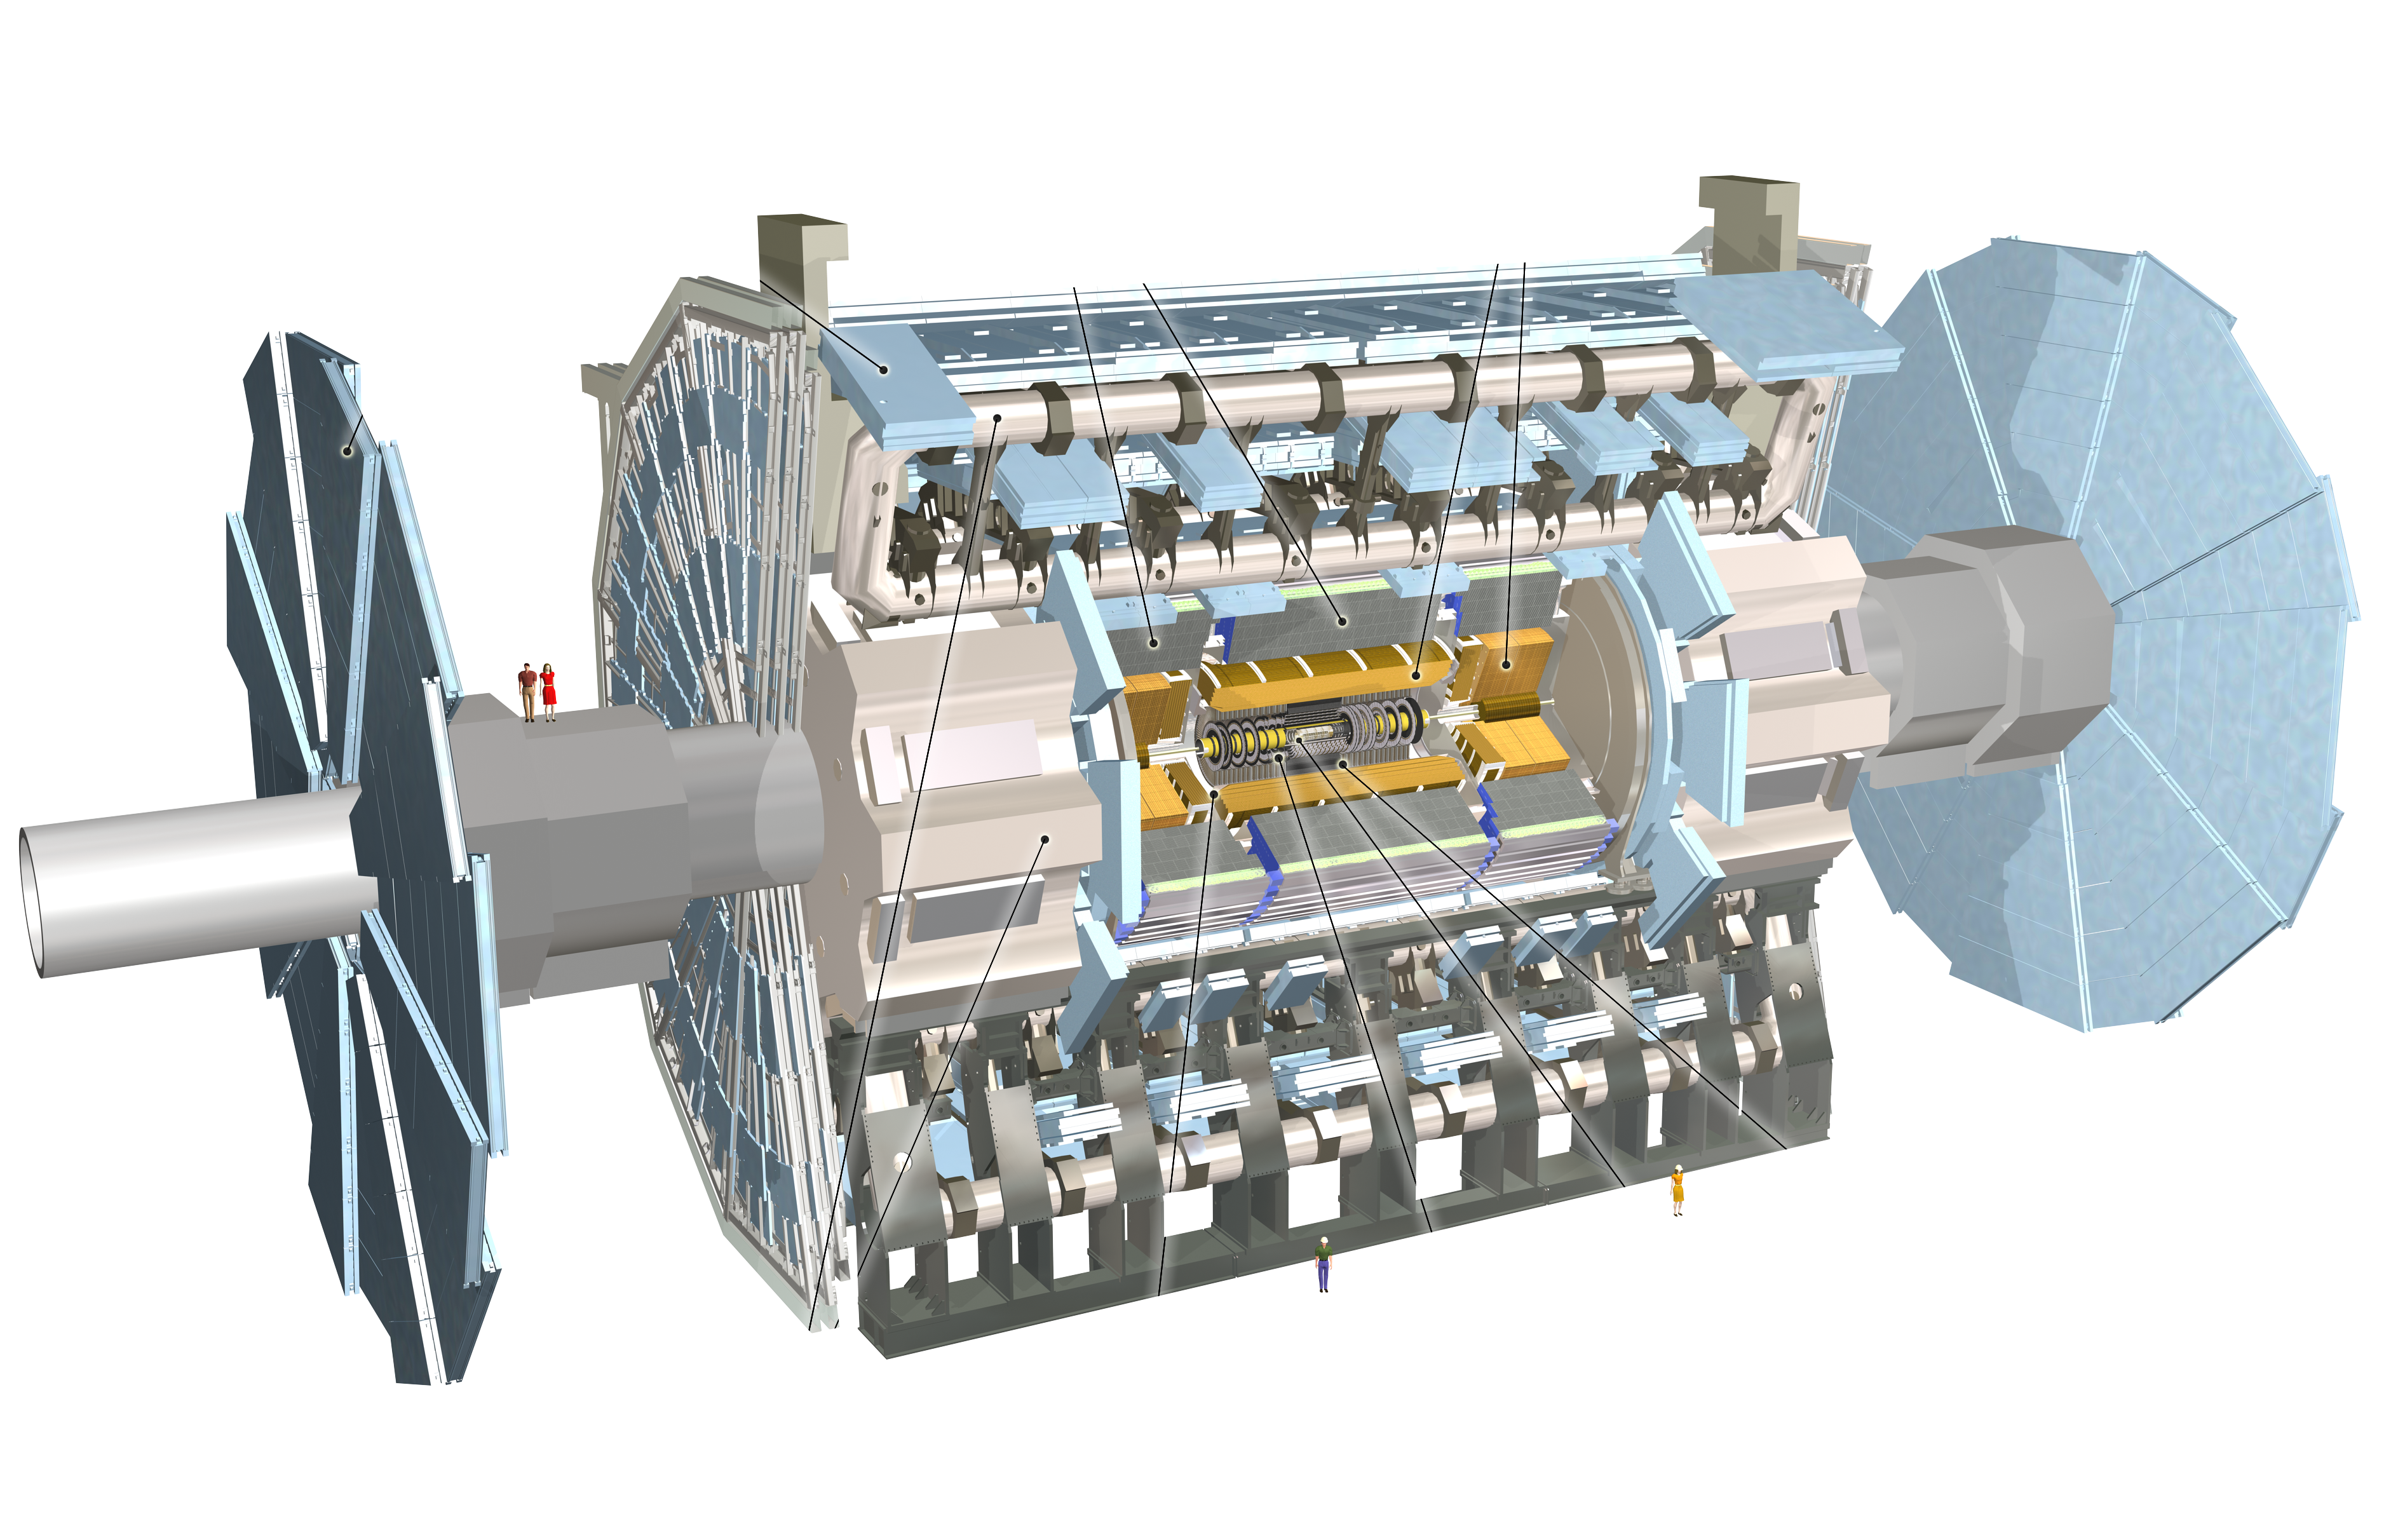
\includegraphics[width=0.95\textwidth]{all_atlas}
\caption{ }
\label{fig:exp.sumLumiByDay}
\end{figure} 





%% Number of Interactions per Crossing
%% Shown is the luminosity-weighted distribution of the mean number of interactions per crossing for the 2016 pp collision data at 13 TeV centre-of-mass energy. All data delivered to ATLAS during stable beams is shown, and the integrated luminosity and the mean mu value are given in the figure. The mean number of interactions per crossing corresponds to the mean of the poisson distribution of the number of interactions per crossing calculated for each bunch. 
%% The preliminary luminosity measurement is used to determine the number of interactions per beam crossing as $mu = L_\text{bunch}  \sigma_\text{inel} / f_r$ where $L_\text{bunch}$ is the per-bunch instantaneous luminosity, $ \sigma_\text{inel} $ is the inelastic cross-section at 13 TeV, which is taken to be 80 mb, and $ f_r$ is the LHC revolution frequency of 11.245 kHz.
%%  The luminosity shown represents the preliminary 13 TeV luminosity calibration released in February 2017, based on van-der-Meer beam-separation scans in 2016.
